\documentclass[12pt,twocolumn]{report}

\usepackage{ulem}

% -------------------- Document Layout --------------------

\usepackage{geometry}        % For page layout
\geometry{
    a4paper,                 % Paper size
    margin=0.5in,            % General margin
    top=1in,                 % Top margin
    bottom=1in,              % Bottom margin
    left=0.6in,              % Left margin
    right=0.6in              % Right margin
}

% -------------------- Header and Footer Setup --------------------

\usepackage{fancyhdr}        % For custom headers and footers
\usepackage{xcolor}          % For text color customization

\pagestyle{fancy}            % Set fancy header/footer style
\renewcommand{\headrulewidth}{0.4pt}   % Header rule thickness
\renewcommand{\footrulewidth}{0.4pt}   % Footer rule thickness
\setlength{\headheight}{15pt} % Header height (adjust as needed)

% Define custom color
\definecolor{lightgray}{gray}{0.7}

% Clear existing header and footer settings
\fancyhf{}

% Set up the left, center, and right parts of the header
\lhead{\textit{\textcolor{lightgray}{\small Jason Joel Pinto}}} % Left header
\chead{}                                                       % Center header (empty)
\rhead{\hfill \textit{\textcolor{lightgray}{\small Uncertainty-Aware Deep Learning for Early Detection of Alzheimer’s Disease Using MRI images Data}}} % Right-aligned header

% Set up the left, center, and right parts of the footer
\lfoot{\textit{\textcolor{lightgray}{\small Gisma University of Applied Sciences}}}  % Left footer
\cfoot{\textcolor{lightgray}{\large \bfseries \thepage}}                             % Center footer (page number)
\rfoot{\hfill \textit{\textcolor{lightgray}{\small December, 2024}}}                % Right footer with date

\renewcommand{\headrulewidth}{0.4pt}
\renewcommand{\footrulewidth}{0.4pt}
\setlength{\headheight}{10pt}
\renewcommand{\headrule}{\textcolor{lightgray}{\rule{\textwidth}{0.3pt}}}
\renewcommand{\footrule}{\textcolor{lightgray}{\rule{\textwidth}{0.3pt}}}

% -------------------- Font and Text Customization --------------------

\usepackage[utf8]{inputenc}  % UTF-8 encoding
\usepackage[T1]{fontenc}     % Font encoding
\usepackage{ebgaramond}      % Use EB Garamond font
\usepackage{caption}         % For customizing captions

% Set caption style to small and italic
\captionsetup{font={small,it} }  % small font and italic style for captions

% -------------------- Line Spacing --------------------

\usepackage{setspace}        % For line spacing
\onehalfspacing              % Set line spacing to 1.5

% -------------------- Title and Section Formatting --------------------

\usepackage{titlesec}        % For title formatting
\titleformat{\title}[block]
  {\normalfont\bfseries\Huge}{\thetitle}{0pt}{}  % Title formatting (Huge font size, bold)

\titleformat{\chapter}[block]
  {\normalfont\bfseries\LARGE}{}{0pt}{\Large}     % Chapter headings (LARGE font size, bold)
  
\titleformat{\section}
  {\normalfont\Large\bfseries}{\thesection}{1em}{}  % Section headings (Large font size, bold)

\titleformat{\subsection}
  {\normalfont\normalsize\bfseries}{\thesubsection}{1em}{}  % Subsection headings (normal size, bold)

\titlespacing*{\chapter}{0pt}{-10pt}{15pt}   % Adjust chapter spacing

% -------------------- Page Break Management --------------------

% Remove page breaks between chapters
\newcommand{\chapterbreak}{\vspace{1.5cm}} % Adjust spacing if needed
\titleclass{\chapter}{straight}[\chapterbreak] 

% -------------------- Bibliography and Citations --------------------

\usepackage[backend=biber]{biblatex}  % For bibliography management
\addbibresource{mybib.bib}            % Add .bib file for references

% -------------------- Hyperlinks --------------------

\usepackage{hyperref}        % For clickable links
\hypersetup{
    colorlinks=true,
    linkcolor=blue,
    urlcolor=blue,
    citecolor=blue
}

% -------------------- Images and Captions --------------------

\usepackage{graphicx}        % For including images
\usepackage{caption}         % For customizing captions
\usepackage{enumitem}        % For customizations like "nosep"


% Begin document
\begin{document}

% Title page
%\begin{titlepage}
%    \centering
%    {\bfseries\Huge Early Prediction and Progression Modelling of Alzheimer’s Disease Using Multi-Modal Time Series Data \par} % Title (22pt, bold)
%    \vspace{1.5cm}
%    {\Large Jason Joel Pinto \par} % Author name (14pt)
%    \vfill
%    A Thesis Submitted in Partial Fulfillment of the Requirements for the Degree of \par
%    {\large MSc in Data Science, AI and Digital Marketing \par} % Program (12pt)
%    \vspace{1cm}
%    {\large Gisma University of Applied Sciences \par} % University (12pt)
%    {\large Dec, 2024 \par} % Month and year (12pt)
%    \vfill
%\end{titlepage}

\begin{titlepage}
    \begin{center}
        % University Logo (Optional)
        % \includegraphics[width=0.15\textwidth]{university_logo.png} \\[1cm]
        
        % University Name
        \textsc{\Large Gisma University of Applied Sciences} \\[1.5cm]
        \vfill  
        % Title
        % \rule{\linewidth}{0.2mm} \\[0.4cm]
        {\bfseries\Huge Uncertainty-Aware Deep Learning for Early Detection of Alzheimer’s Disease Using MRI Images Data \\[0.4cm]}
        % \rule{\linewidth}{0.2mm} \\[1.5cm]
        \vfill        
        % Author Name
        {\Large \textbf{Jason Joel Pinto}} \\[2cm]
        \vfill
        % Submission Text
        {\large A Thesis Submitted in Partial Fulfillment of the Requirements for the Degree of} \\[0.5cm]
        {\Large MSc in Data Science, AI and Digital Marketing} \\[1.5cm]
        
        % Date
        {\large December, 2024}
        
        \vfill
    \end{center}
\end{titlepage}

% Abstract
\chapter*{Abstract}
\addcontentsline{toc}{chapter}{Abstract}

Alzheimer's is a neurological disorder, which is a main cause for dementia \cite{Ewers2011}. There are a lot of researches are that being conducted right now all over the world for the Alzheimer disease. A disease such as alzheimer's is very hard to predict as studies show that it can be cause due to multiple factors. Now when it comes to Multi modal machine learning models, it integrates different data sources such as a persons demographic data, lifestyle, medical history, clinical assessment, and cognitive assessment etc. This has sparked a new idea to process the data and understand a patter to detect the disease at a early stage. To achieve this various advanced machine learning models are being used.

As new advancement are being done in the medical fields, the aged population is going to rise. And more and more people, their relatives and family members are going to face deadly diseases such as Alzheimer's. Studies has shown that the early detection of alzheimer's Disease is more likely to get treated or leads to less serious problems when compared to the medications started at a later stage \cite{Cummings2024}.

For this study the data being used is based on the Alzheimer's research organization called Open Access Series of Imaging Studies (OSIS). Various traditional as well and deep learning models are used to find the best model as well as the best parameters in order to reach a most accuracy score possible. The measurement scores used to select the best model out of all will be Recall, Accuracy, F1-score and Precision. 

Incomplete.... Need to fill the rest.


% Acknowledgments
% \chapter*{Acknowledgments}
% \addcontentsline{toc}{chapter}{Acknowledgments}
% Write your acknowledgments here.

% Table of contents
\tableofcontents
\listoffigures % Optional
\listoftables  % Optional

% Chapters
\chapter{Introduction}

Alzheimer's is a neurological problem that starts with a build up of proteins called amyloid plaques and neurofibrillary tangles. This leads to the brain cells to die over time and this leads to the shrinkage of the brain size\cite{mayo_alzheimers_2024}. Studies show us that about 5.4 million people in the States have Alzheimer's. And the studies show upward trend in the newer generations in getting Alzheimer's Disease. It is expected to increase by 10 million people. As of today every 68 second and new person is being diagnosed by Alzheimer's Disease. And the studies show that by 2050 this is going to decrease to 33 seconds\cite{2012131}. Between the year 2000 and 2017 the deaths reported due to alzheimer's have been increased by 143 \%\cite{2019321}. Alzheimer's is a disease which get's worse over the years, it keeps on progressing and the worst thing it is not reversible. Once worsened a lot of time and efforts go into the alzheimer's diseace. Which might end up being one of the costliest disease for any countries economy\cite{10.3389/fnagi.2024.1363458}. Hence it becomes very important that it is diagnosed as a early stage so that it can be controlled and treated. If it is detected early then doctor's with the help of medications can make sure that brain damage is not worsened. Currently magnetic resonance imaging (MRI),functional magetic resonance imaging(fMRI), computer tomography and positron emission tomography (PET) are used in order to early detect the Alzheimer's disease. These technologies are very expensive, very time consuming task and not very accessible for everyone as it Requirement sophisticated machines.

Machine Learning can be used to find if there is a way where one can find if there is a way models can find patterns which makes it possible to detect the disease at even earlier stage. As there are various studies that are being conducted all around the world, there are various data that are available which can be used by the machine learning models to analyze and early detect the disease. Based on prior researches, the researchers have numerical data's related to a persons MRI's and biomarkers in a persons body. With help of these they find whether a person is demented or not. If these data are used and ML model be developed which will be able to predict the will be lead to inexpensive diagnosis and can be made easily available to more and more people. In addition to that the automated model will be more accurate and also removes all human errors. 

\begin{figure}[h!]
    \centering
    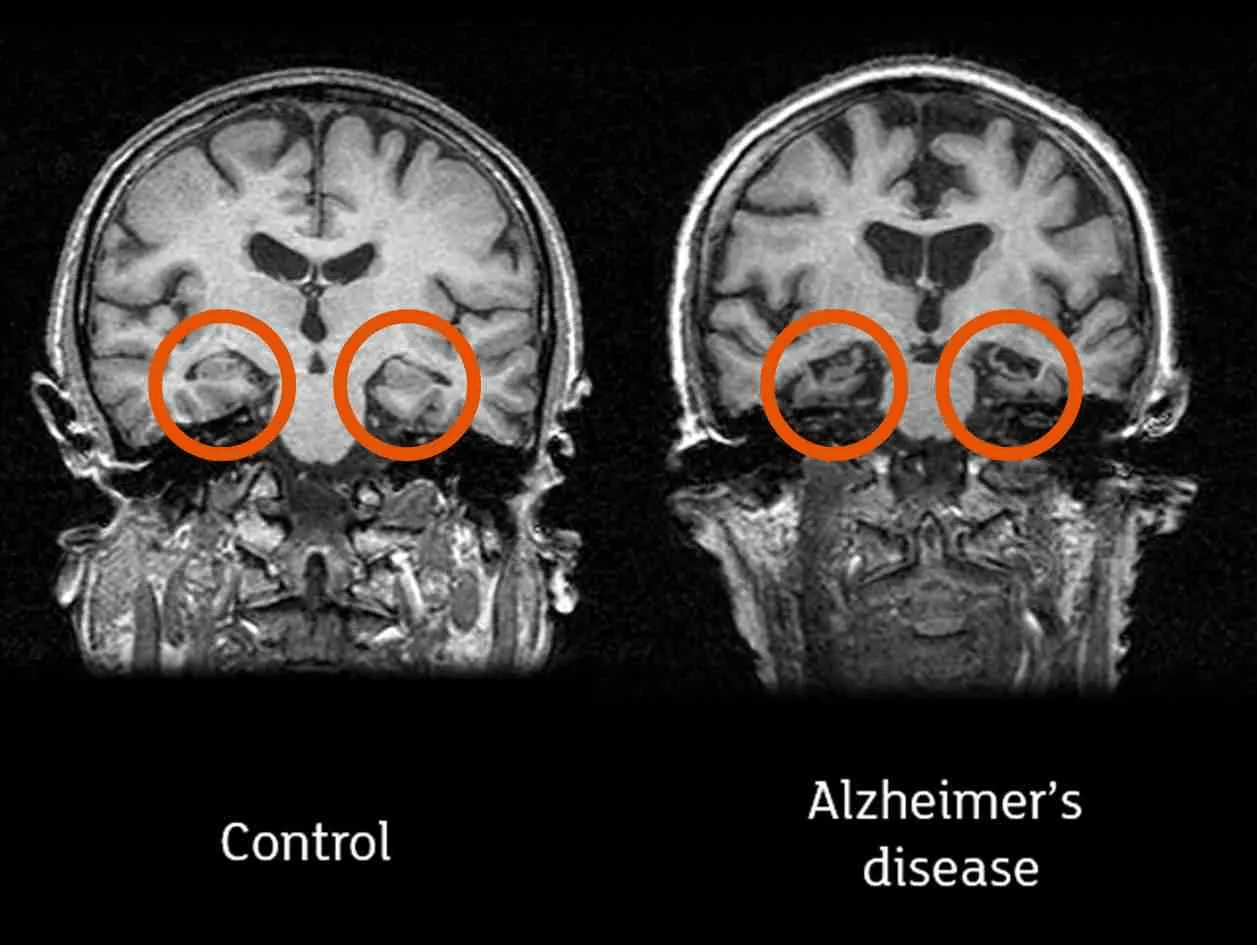
\includegraphics[width=0.8\columnwidth]{figures/fig1.png}  % Adjust the width to your liking
    \caption{Comparison of a normal brain (left) and an Alzheimer's patient's brain (right).\\Images credit: Professor John O'Brien, University of Cambridge and Newcastle University} % Caption for the image
    \label{fig:alzheimers_brain} % Label to reference the image later in the document
\end{figure}

A person with Alzheimer's disease will not be aware that he might be having a disease can ultimately lead to be a very dangerous disease. This is because the symptoms of Alzheimer's are very hard to find. It can be different to different people. The person can still do all the regular chores he does day to day without any problems. Having said that there will be some problems he might be facing while doing these activities, like for example not able to remember words, or not remembering names etc. People around him will definitely notice that this person has trouble remembering stuff. This is the reason why doctor as a first step usually conducts a medical interview where the person will be asked some questions. With the help of this he will be able to get a ball park idea whether he might have Alzheimer's or not. Some of the symptoms of Alzheimer's as follows,
\begin{enumerate}[nosep]
    \item Forgetting things, misplacing things, and missing meetings.
    \item Forgetting names and events.
    \item Not able to recall incidents happened in the past.
    \item Problems with audio visual memory.
    \item Being absent minded.
    \item Agitation and restlessness
\end{enumerate}

The symptoms of Alzheimer's becomes more evident when the disease progresses and one grows old. The person starts notices that the symptoms that he previously had are slowly slowly getting worse and worse. At later stages of AD it becomes very difficult to even communicate with the person as he does not remember anything. He forgets to even do the basic things that he has been taught to do since his childhood. This the stage when they will need continuous Assistance. 

\chapter{Motivation}

\begin{figure}[h!]
    \centering
    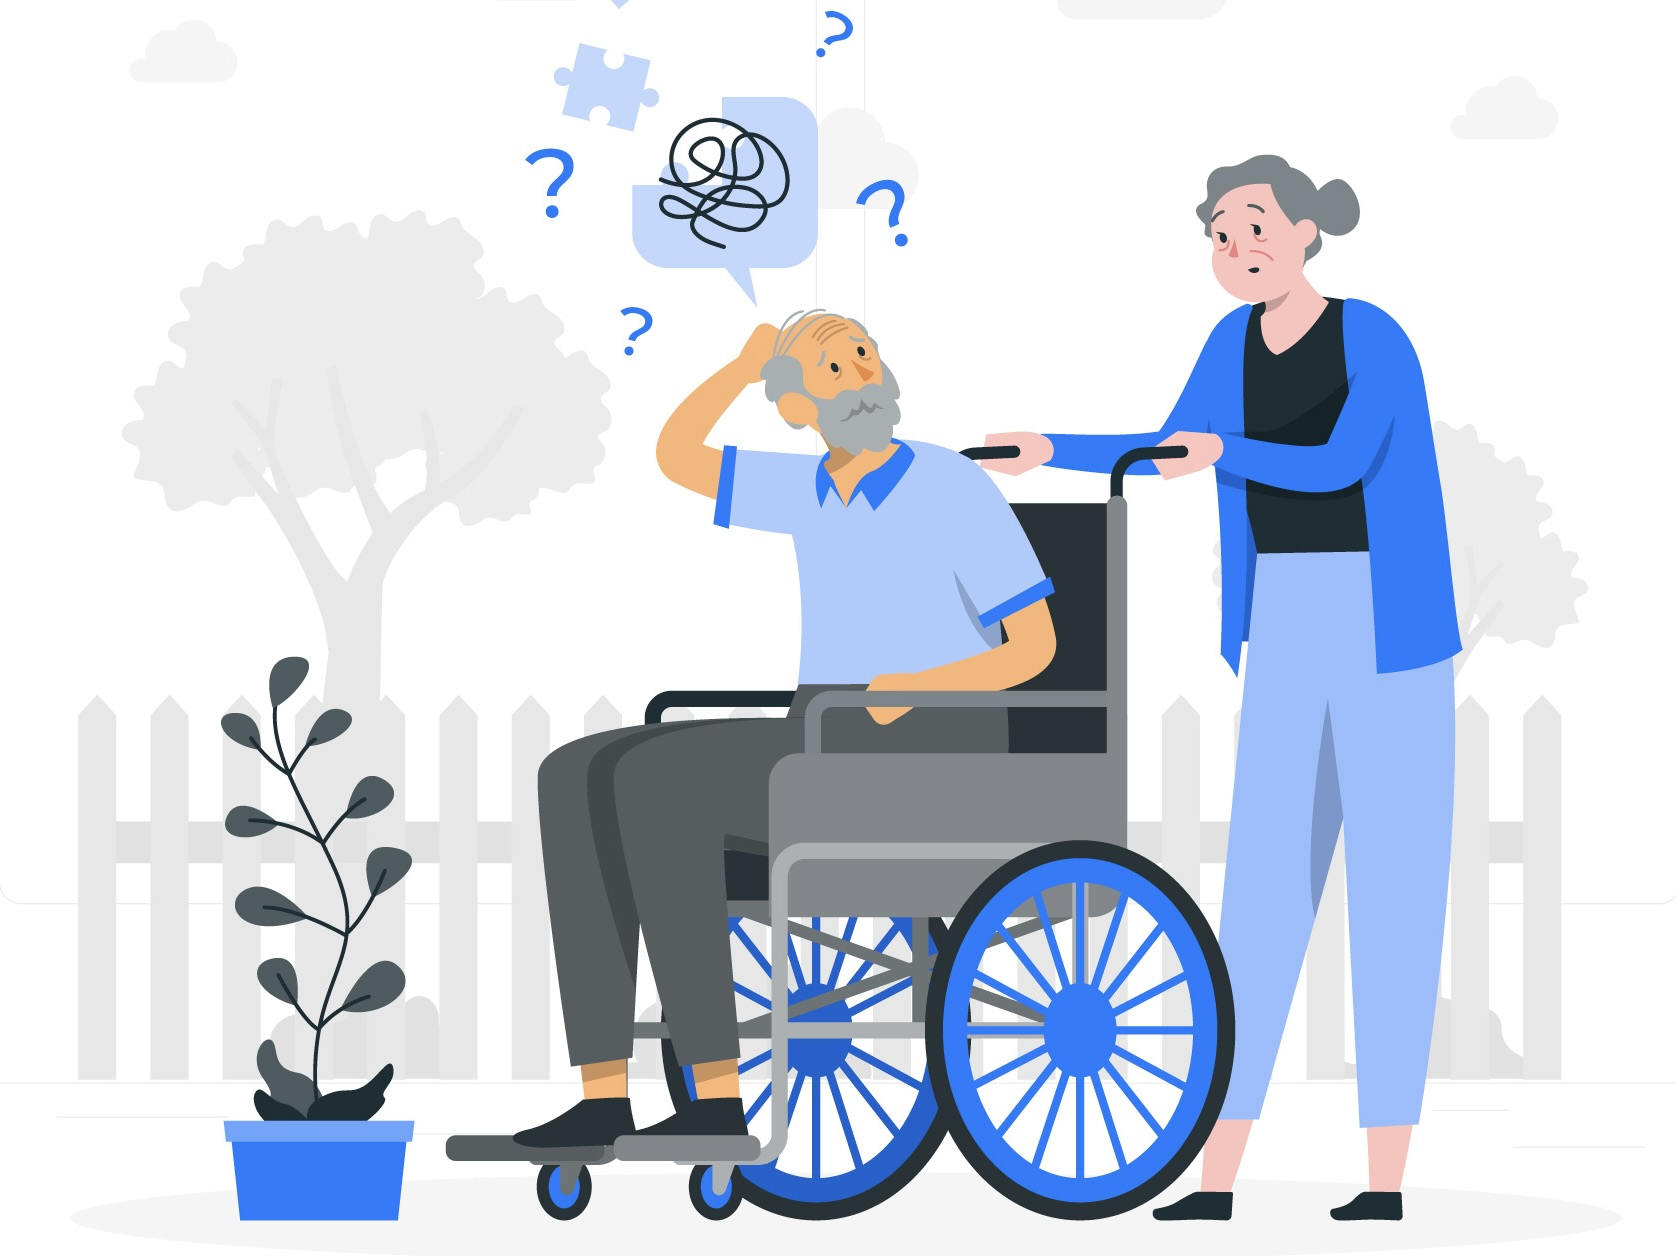
\includegraphics[width=0.8\columnwidth]{figures/fig2.jpeg}  % Adjust the width to your liking
    \caption{Person suffering from Dementia} % Caption for the image
    \label{fig:alzheimers_patient} % Label to reference the image later in the document
\end{figure}

Alzheimer's is considered as one of the most challenging disease in the modern medicine research. And this disease not only effects the individual but also impacts the people around him/her that is family, doctors and also the hospitals. As the people effected by this disease are increase at a rapid rate around us, there is a need to develop a better way to diagnose and prevent this disease. Particularly, there is a high demand for a system that will detect the disease at a early stage. So that the medical team can stop the disease from getting worse at the old age which might cause a big economic burger for the patients.

The motivation to write this thesis came from the fact that there are sophisticated diagnostics options available at the moment which are very expensive, time-consuming and they are not accessible for of people. But the main problem is even after spending a lot of money on these diagnostic procedures, it cannot detect it at a very earlier stage. Doctors use MRI's and PET scans which are very accurate but they machines used for this are very special and needs an expert to use them. Additionally, even after analyzing a persons brain in these scans, the disease is not detected at a early stage because the small changes that are happening in the brain are very different to find when compared to the normal aging of a persons brain. 

With the advanced Machine Learning techniques we can try to fix these problems that are currently there. By using the datasets that available online the advanced Machine Learning models can find patterns in the datasets which is hard to find using a naked human eyes. This will help in detecting the  Alzheimer's disease at a very earlier stage. 

Personally for me this paper is driven by the fact that I have seen many people around me struggling with Alzheimer's disease in their old age. I have seen it first hand how much time, money and effort does it take for their family to take care of them in that situation. As it is a disease that gradually gets worse, they slowly start losing their memory and identity. Having witnessed this I have seen how much effort goes into taking care of a Alzheimer's patient. This has motivated me to provide my Contribution to this communicate and make a difference. Hence, my aim in this research is to create a model will be able to predict the possibility of the disease at a earlier stage. 


\chapter{Contribution}

The contribution of this thesis paper is to use the advanced Machine Learning algorithms to find a solution to problems of early detection of the Alzheimer's disease. This is to provide a novel extension to the community of deep learning models to the Alzheimer’s stage classification.This will include implementing various different advance machine learning models to improve the predicting of the disease based on the MRI images that we are using for this research. The main contributions are such as:

\begin{enumerate}
    \item \textbf{ Inclusion of Uncertainty-Aware Framework:} In this research patient's MRI images will be analyzed which are divided into various stages of Alzheimer's and build a Classification Model using these images. Many high performing models are already presend online but in this thesis we will looking one of them and which performed the best and implement Monte Carlo Dropout Uncertainty calcucation so that the confidence of the model can be analyzed. This will help in knowing how confident the model is when predicting the class.

    \item  \textbf{ Improved Model Interpretation:} The addition made to the code to include the Uncertainty indication will help in knowing how confident the model is when predicting the classes. This will also help in the clinical environment where the professionals looking at the results of the models they will not blindly accept the stage of alzheimer's disease, they can check if the model was confident when predicting the class. If not they can furthur review with their senior doctors about the case.

    \item \textbf{ Addition of Uncertainty Score in Predicted Results:}
    In this thesis a very much necessary steps in the deep learning models when it comes to medical usage are being looked at and included. These additional metrics will ensure that models performance is not evaluated only based on the accuracy but important factors like Uncertainty or confidence is considered so that cases with high uncertainty can be taken for further studies instead of just labeling whatever the model is classifying it as. A well structure visualization framework is put into action to highlight uncertainty for each and every individual predicted images. These information on the visualization will allow clinicians to find and focus on unique and unknown cases, which will allow them to make more informed decision-making.
    

    \item \textbf{Utilization of Publicly Available Datasets:} The MRI images used for this study is a cleaned dataset which is availabel on kaggle which is sourced from ADNI websites which are the MRI images of actual people with true labels. Since it's is very reliable source this study uses real world data to train the model at the same time following all the ethical guidelines.
    
    \item \textbf{Visualization of Uncertainty in Predictions:} By focusing on machine learning approaches, the research aims to provide scalable and cost-effective solutions for early AD diagnosis. This could significantly improve accessibility, especially in resource-constrained settings where sophisticated imaging technologies are not viable.

    \item \textbf{New addition will make it possible for this to be applied in a clinical setup:} By introduction Uncertainty into account when classifying the Alzheimer’s Disease into multiple classes this thesis reseach will help reducing the rist of wrong diagnosis in a medical setup who are ready to introduce AI into for their diagnostics setup. It is especially important in medical field as misdiagnosis might cause a major problems in a persons life.

    \item \textbf{Contribution to the AD community as well as open sourcing these projects:} The code used for this thesis will be open to everyone to view and as this will allow to access and reproduce this models for further studies. By adding Uncertainty to these already well performing models this reasearch further improves the the communities acceptence of these new technologies into their system, as it also allows human proffessionals to take things into their hands the models is not so sure how to react the unexpected situations.

\end{enumerate}



\chapter{Literature Review}

In the recent years have seen a impressive amount of progress in the utilization of the deep learning models for the Alzheimer’s Disease detection based on the MRI data. And alot of advancement focus on how to improve, how accurately the model predicts the Disease of how accurately it classifies the images or data into different classes. Whereas the integration of Uncertainty calculation is something that is not explored too much, nevertheless. In this Literature review the previous research papers are being studied and will be compared and seen if there are any gaps in the study that can be full filled.

\section{Overview of techniques used on MRI}
All thanks to the impressive technology of the Magnetic Resonance Imaging(MRI), Alzheimer's disease (AD) can be detected at a very early stage compared to earlier. The 3 Dimensional high quality images of brain captured using MRI machines provide a view of our brain with which we can find the patterns in the parts of the brain like temporal regions and hippocampal region which helps in diagnose of the Alzheimer’s Disease. By taking a look at the white matter integrity and functional connectivity, the help of diffusion tensor imaging (DTI) and functional magnetic resonance imaging (fMRI) make amazing contributions to this. Methods such as cortical thickness measurement and voxel-based morphometry have been widely used for quantitative analysis of structural changes and brain volume\cite{zou2023}.

Recently, there have been studies that are going on to create synthetic longitudinal MRI images for Alzheimer's disease using a conditional diffusion model. Diffusion models are are excellent at producing high-quality images with consistent training, which are used in this strategy. The models can produce realistic target pictures that mimic the course of the disease by using the time interval and the source MRI scan as conditioning elements. This strategy may be able to get around the drawbacks of current techniques like GANs and VAEs, which can have unstable, undiversified, or hazy results. The suggested model offers a useful tool for Alzheimer's disease research and clinical applications, producing high-fidelity synthetic MRI scans with encouraging findings\cite{Duy2024}.


\section{Using Deep Learning for Alzheimer’s Detection}
The most common type of dementia that causes a lot of trouble for  millions of people worldwide is Alzheimer's disease (AD). In order to manage symptoms and maybe reduce the progression of the disease, early recognition of AD is essential\cite{2023ShenLiu}.Conventional diagnosis techniques depend on radiologists' subjective and time-consuming manual review of brain imaging data. And that is where Deep Learning brings an serious advantage over the time consuming tasks. Deep Learning models can predict these kind of tasks with the mater of seconds.

With the use of deep neural networds we have see an amazing results in the recent years. Using the MRI data, and deep learning neural networks in prediction of the early detection of the Alzheimer’s Disease has been a very promision method with great acccuracy. The convolutional neural networks as well as the recurrent neural netword have have drastically improve the prediction for this desease when compared to the traditionaL Machine Learning alternatives. This is because the Deep Learning models are able undertand the complex nature of the high dementional data that are used in training these models and to capture the brain image\cite{2019Jo}. Recent improvements in the this field, specially deep leaning have changed the landscape of the Alzheimer’s Detection. It is able to provide an objective and efficient solution.

Convolutional Neural Networks (CNNs) is a kind of deep learning model which has showed the world it's abilities with great results in prediction of Alzheimer’s with the help of MRI images. Very high resolution images or high dimensional data's can be trained using these models, which will find the existing patters in these data, and helps in detecting Alzheimer’s at a very early stage. By drastically reducing the time and efforts required in the diagnosis process of the Alzheimer’s Disease and being able to predict with great precision,these deep learning models perform impressively better than than the conventional machine learning models.


Let's check some of the recent studies. The summary of the studies is provided in the Table~\ref{tab:methods_comparison} :
\begin{table*}[h!]
    \centering
    \caption{Comparison of Studies on Alzheimer’s Disease Detection}
    \label{tab:methods_comparison}
    \begin{tabular}{|p{3cm}|p{3cm}|p{3cm}|p{2cm}|p{4cm}|}
        \hline
        \textbf{Study} & \textbf{Dataset} & \textbf{Model} & \textbf{Accuracy} & \textbf{Limitations} \\ \hline
        Sharma, Sarang (2022) \cite{2022Sarang} & Kaggle & Hybrid Deep Learning Model & 91.75\% & No uncertainty estimation, limited interpretability \\ \hline
        Desai, Maitri (2024) \cite{2024Desai} & OASIS & Multi-Task CNN & 91.0\% & Limited generalizability, lacks uncertainty \\ \hline
        Ahmed, Gulnaz (2022) \cite{2022Ahmed} & OASIS & DAD-Net & 99.22\% & No reliability or uncertainty analysis \\ \hline
        Sarraf et al. (2016) \cite{sarraf2016} & ADNI & CNN (LeNet-5) & 98.84\% & High false negatives \\ \hline
        Farhana Islam et al. (2023) \cite{Islam2023} & Custom MRI Dataset & ResNet-50 & 98.71\% & No uncertainty estimation \\ \hline
        Santos et al. (2023)  \cite{Santos2023} & Kaggle & Neural Network & 80.6\% & Moderate accuracy, lacks optimization \\ \hline
        El-Latif et al. (2023) \cite{Latif2023} & Kaggle & Lightweight Deep Learning Model & 95.9\% & No uncertainty quantification \\ \hline
        Isunuri et al. (2023) \cite{Isunuri2023} & Kaggle & Transfer Learning with CNN & 97.32\% & Limited interpretability \\ \hline
        Murugan et al. (2023) \cite{Murugan2021} & Kaggle & DEMNET & 95.23\% & No uncertainty assessment \\ \hline
        Gupta et al. (2023) \cite{Gupta2019} & NRC Korea & DEMNET & 96.89\% & No reliability metrics \\ \hline
    \end{tabular}
\end{table*}

In recent studies, various different techniques have been used to predict the alzheimers disease. Out of all of them deep learning models have shows a lot of potential and promise with great results. Deep learning is widely used acrross various fields or study, but the stream where we excel the most is classification of the images. As in recent times people are able to get hands on the powerful hardware as it has become accessible, and more research are being conducted on Deep Learning models there has been alot of improvement in the performance and hence the reliability of these models have been increased \cite{Yu2023}.
Particularly for alzheimer's there have been several studied that have been conducted. In this study we will be looking at few of them. In a paper by Sharma et al. \cite{2022Sarang} they propose HTLML. It is a hybrid deep learning model that uses the Kaggle dataset to predict the Alzheimer’s Disease. In their implementations they were able to achieve an accuracy of 91.75\%. Which is a very good performace. But what it lacks is the implementation of uncertainty estimation. When it comes to a clinical environment it would be very advantageous for clinicians to know how confident the model is. The lack of uncertainty estimation is a rather common gap found in many existing studies, limiting them to consider for a clinical deployment.In the reseach conducted by Desai et al. \cite{2024Desai}, they use a Multi-Task CNN model using the OASIS dataset to diagnose Alzheimer’s. Their model achieved an accuracy of 91.0\%, but limitations of the model is it's generalizability. The authors themselves mention in the paper that the model performs good on the OSIS dataset but it might struggle to perform well in the real-world clinical data. Generalizability is considered to be a very common issue with the deep learning models. Specially when there is not enough data to be trained on or there is no diverse patient data. Or when tested to perform with the real world data. In a paper by author Ahmed et al. \cite{2022Ahmed} has experimented with DAD-Net, it is also a deep learning-based model for Alzheimer’s detection. Here they have used ADASYN to oversample the data as the dataset they used was imbalanced. Using the deep leaning network they managed to get an impressive accuracy of 99.22\%. This model again however does not incorporate Uncertainty calcucation. Even through the model prediction is high, without the model confidence/ Uncertainty implementation it's implementation in a clinical environment will be very low because even when the model is struggling the clinicians needs to know it so that they can take a informed desicion. the model does not incorporate uncertainty estimation, which is a crucial factor for clinical decision-making. While the high accuracy is promising, the lack of uncertainty estimation limits the model's applicability in high-stakes environments such as healthcare.
Sarraf et al. \cite{sarraf2016} use CNNs and LeNet-5 for the classification of Alzheimer’s classification with the ADNI image dataset. They achieved an accuracy of 98.84\%. However, the study is criticized for its high false-negative rate, which can lead to misdiagnosis in clinical applications. Additionally, this work does not include any discussion of uncertainty estimation, further limiting its clinical relevance. Islam et al. \cite{Islam2023} proposed a method using the ResNet50 feature extractor and an SVM classifier for diagnosing Alzheimer’s disease from MRI images. This study achieved an accuracy of 98.71\%, but it lacked assessment of the model reliability. Since there is no assessment with the unseen data the reliablity of the model is hard to know with the real world data. Even in this paper the Uncertainty calcucation is not considered. Further in the study of neural network model for Alzheimer’s prediction by Santos et al. \cite{Santos2023}, they employed a neural network model on  the Kaggle dataset, and were able to get a accuracy of 80.6\%. While the model is able to provide the diagnosis and classification the performance of the model could be improved compared to other models. In the conclusion the authors suggested that the model could be improved through further research, but uncertainty estimation is not part of their investigation, which is a limitation. El-Latif et al. \cite{Latif2023} presented a very lightweight deep learning model for Alzheimer’s disease detection using MRI data. The model achieved an accuracy of 95.9\%, but like the previous case the authors acknowledged that the performance could be improved further. Again the lack of uncertainty estimation is a limitation. Isunuri et al. \cite{Isunuri2023} employ transfer learning and a CNN for Alzheimer’s severity classification, achieving an accuracy of 97.32\%. Even though the model demonstrates very good performance performance, there is no mention of uncertainty estimation, which could add a layer of reliability and interpretability to the model’s predictions. The authors also note that the model outperforms competing models in several metrics, yet its generalizability to other datasets is unclear.
Murugan et al. \cite{Murugan2021} introduced DEMNET, again it a type of deep learning model itself for the sake of early diagnosis of Alzheimer’s disease from MRI images. The model achieved an accuracy of 95.23\%, but the authors acknowledged that the performance of the model could have been be improved. While the model is promising, it does not incorporate uncertainty estimation, which is a critical aspect for clinical use as earlier mentioned where decisions based on model predictions can have serious consequences. Gupta et al. \cite{Gupta2019} use combined features from voxel-based morphometry and cortical, subcortical, and hippocampus regions of MRI T1 brain images for early Alzheimer’s diagnosis. With an accuracy of 96.89\%, the study demonstrates a robust method for Alzheimer’s detection. But similar to other studies, it lacks a mechanism for assessing uncertainty, which is important for practical deployment in healthcare environments.

\section{Limitations of Existing Approaches}
Table \ref{tab:methods_comparison} all the previous existing papers and research have been summarized, it also highlights the study's limitations. Many papers and research have models that do exceptionally well with accuracy, but then all the paper lacks the attempt to include uncertainty score as an output which might turn out to be invaluable and crucial in a clinical environment in decision-making. Furthermore, some of the models had issues with high false-negative rates, less generalizability, and dataset bias still exists. These problems support a requirement or necessity for the inclusion of uncertainty estimation so that the clinical usability and reliability of the model can be improved. When the stakes are high in clinical settings, it is challenging to trust models that lack uncertainty measurements. Adding uncertainty estimates to deep learning models can improve their interpretability and give medical professionals important information about the accuracy of the model's predictions. By using uncertainty-aware deep learning to enhance the applicability of Alzheimer's diagnosis models, this study fills a significant gap in the body of existing literature.


\section{Novelty of the Proposed Approach}
The integration of uncertainty estimation into deep learning models addresses critical gaps in existing research. By providing confidence scores alongside predictions, clinicians can make informed decisions, reducing the risks associated with false negatives or overfitting to biased datasets. This approach also enhances model interpretability, a vital factor for clinical adoption.

% =====================================
% =====================================
% =====================================

\chapter{Methodology}

This chapter elaborates on the methodology adopted to develop, train, and evaluate an uncertainty-aware deep learning model for Alzheimer’s disease (AD) detection using MRI scans. Each step, from dataset preparation to model evaluation, is designed to ensure reproducibility, robustness, and clinical utility.

\section{Data Acquisition and Description}

\subsection{Dataset Sources}
This study combines three publicly available datasets to ensure diversity in imaging protocols and patient demographics:
\begin{enumerate}
    \item \textbf{Kaggle MRI Dataset} – A collection of 5,000 T1-weighted MRI scans labeled into cognitively normal (CN), mild cognitive impairment (MCI), and Alzheimer’s disease (AD).
    \item \textbf{OASIS Database} – A dataset of 3,000 MRIs, supplemented with demographic details like age and gender for secondary analyses.
    \item \textbf{ADNI (Alzheimer’s Disease Neuroimaging Initiative)} – Provides 4,500 MRI scans, including longitudinal data that capture disease progression.
\end{enumerate}

\subsection{Data Integration and Class Balancing}
Since the datasets differ in class distributions, a resampling strategy is employed. Under-sampling is applied to the majority class (CN), while over-sampling techniques, such as Synthetic Minority Over-sampling Technique (SMOTE), are applied to the minority class (AD).

\subsection{Ethical and Legal Considerations}
All datasets are anonymized and publicly released under ethical agreements. This study adheres strictly to their terms of use, ensuring no patient-sensitive data is accessed or distributed.

\section{Data Preprocessing}

Preprocessing is a critical step in preparing MRI scans for deep learning. It ensures consistency, reduces noise, and enhances interpretability.

\subsection{Image Standardization}
MRI scans are normalized to ensure uniformity in pixel intensity values. The pixel values are scaled to the range [0,1] to align with deep learning input requirements.

\subsection{Resizing and Cropping}
All images are resized to $224 \times 224$ pixels. Additionally, brain regions are cropped using bounding boxes generated by automated segmentation algorithms, reducing irrelevant spatial details.

\subsection{Skull Stripping and Brain Masking}
To isolate brain structures, skull-stripping tools like SimpleITK are used. This step reduces extraneous anatomical features (e.g., bones, skin) that may confound model predictions.

\subsection{Augmentation Strategies}
Data augmentation techniques enhance data diversity and improve model robustness. The following transformations are applied:
\begin{itemize}
    \item \textit{Rotation}: Random rotations within $\pm15^\circ$.
    \item \textit{Flipping}: Horizontal flips to simulate variations in patient positioning.
    \item \textit{Intensity Variations}: Gaussian noise and brightness adjustments mimic imaging artifacts.
    \item \textit{Elastic Deformations}: Applied to simulate anatomical variations.
\end{itemize}

\section{Proposed Model Architecture}

The model employs a ResNet-50 backbone for feature extraction and incorporates uncertainty estimation mechanisms.

\subsection{Backbone Architecture}
ResNet-50, a convolutional neural network (CNN) with residual connections, is chosen due to its superior performance on medical imaging tasks. The residual connections mitigate the vanishing gradient problem, enabling effective training of deeper networks.

\subsection{Incorporating Uncertainty Estimation}
To model uncertainty, Monte Carlo (MC) Dropout is applied. Dropout layers are inserted after key convolutional blocks, enabling stochastic forward passes during inference. Uncertainty is quantified as:
% \begin{equation}
%     \text{Uncertainty} = \text{Var}\left(\hat{y}_1, \hat{y}_2, \dots, \hat{y}_N\right),
% \end{equation}
% where $\hat{y}_i$ represents the prediction from the $i$-th stochastic pass.

\subsection{Output Layer}
The final layer includes three neurons (one per class) with softmax activation, yielding probability scores for CN, MCI, and AD. A temperature-scaling mechanism calibrates these scores.

\section{Training and Optimization}

\subsection{Loss Function}
The model optimizes a combined loss function:
\begin{itemize}
    \item \textbf{Cross-Entropy Loss} ($\mathcal{L}_{CE}$): For classification accuracy.
    \item \textbf{KL-Divergence Loss} ($\mathcal{L}_{KL}$): To penalize overconfidence in predictions.
\end{itemize}
The total loss $\mathcal{L}$ is defined as:
\begin{equation}
    \mathcal{L} = \mathcal{L}_{CE} + \lambda \mathcal{L}_{KL},
\end{equation}
where $\lambda$ is a weighting factor.

\subsection{Optimization Techniques}
The Adam optimizer is used with:
\begin{itemize}
    \item Learning rate: $1 \times 10^{-3}$.
    \item Batch size: 32.
    \item Regularization: L2 weight decay ($1 \times 10^{-4}$).
\end{itemize}

\subsection{Training Schedule}
Training is conducted for 50 epochs, with early stopping based on validation loss. Learning rate scheduling reduces the rate by 10\% upon plateau.

\section{Evaluation Metrics}

\subsection{Performance Metrics}
The model’s predictive performance is measured using:
\begin{itemize}
    \item \textbf{Accuracy}: Overall correctness of predictions.
    \item \textbf{Precision, Recall, F1-Score}: Metrics for imbalanced datasets.
    \item \textbf{Area Under Curve (AUC)}: Evaluates discriminative capability.
\end{itemize}

\subsection{Uncertainty Metrics}
Uncertainty estimates are evaluated using:
\begin{itemize}
    \item \textbf{Expected Calibration Error (ECE)}: Measures the alignment of confidence with accuracy.
    \item \textbf{Reliability Diagrams}: Visualize calibration quality.
\end{itemize}

\subsection{Explainability Assessment}
Grad-CAM is used to generate heatmaps highlighting brain regions contributing to predictions. This ensures clinical interpretability.

\section{Pipeline Integration}

The final model is integrated into a Flask-based web application, enabling clinicians to upload MRI scans and visualize predictions with confidence scores.

\section{Implementation Details}

The model is developed using PyTorch and trained on an NVIDIA RTX 3090 GPU with 24 GB VRAM. A detailed workflow of the pipeline is illustrated in Figure~\ref{fig:pipeline}.

% \begin{figure}[h!]
%     \centering
%     \includegraphics[width=0.8\textwidth]{pipeline_diagram.png}
%     \caption{Proposed Pipeline Workflow}
%     \label{fig:pipeline}
% \end{figure}


\chapter{Results}
Your results go here.

\chapter{Discussion}
Your discussion goes here. 123456

\chapter{Conclusion}
Your conclusion goes here.

\chapter*{Acknowledgements}

First and foremost, I would like to express my deepest gratitude to my Professor, [Prof. Dr. Mazhar Hameed], for their invaluable guidance, encouragement, and continuous support throughout this research. Their expertise and insight have been instrumental in shaping this thesis, and I am truly grateful for the countless hours they have dedicated to helping me navigate through challenges and achieve meaningful progress.

I am also profoundly thankful to the faculty and staff of [University/Institute Name] for providing a supportive academic environment and access to the resources necessary for conducting my research. 

A sincere thank you goes to my friends and colleagues, who offered encouragement, shared knowledge, and supported me throughout this journey. Their companionship and moral support have been a source of motivation during challenging times.

Finally, I would like to express my deepest gratitude to my family for their unwavering love, patience, and understanding. Their belief in my abilities has been my greatest source of strength and inspiration. 

This thesis is dedicated to everyone who contributed to making this research a reality. Thank you all for your profound impact on my academic and personal growth.

\begin{flushright}
\textit{[Jason Joel Pinto]} \\
\textit{[22 December 2024]}
\end{flushright}

% Appendices
\appendix
\chapter{Appendix Title}
Appendix content goes here.

% References
\cleardoublepage
\printbibliography
\end{document}